\documentclass[12pt]{article}

\usepackage{tgtermes}
\usepackage{epsf}
\usepackage{epstopdf}
\usepackage{amsmath}
\usepackage{graphicx}
\usepackage{booktabs}
\usepackage[colorlinks=true,linkcolor=blue,citecolor=blue]{hyperref}
\usepackage{dcolumn}
\usepackage{amsmath, amsthm, amssymb}
\usepackage{mwe}
\usepackage{url}
%\usepackage{harvard}
\usepackage{fancyheadings}
\usepackage{longtable}
\usepackage{authblk}
\usepackage{setspace}
%\usepackage[nomarkers]{endfloat}
\usepackage{float}
\usepackage{bbm}
%\usepackage{titling}
\usepackage{subcaption}
\usepackage{algorithm}
\usepackage{algorithmic}
\usepackage{import}
\usepackage[backend=biber,style=authoryear,
sorting=ynt,citestyle=authoryear]{biblatex}
\addbibresource{papercitations.bib}
%\usepackage[nomarkers,nofiglist,notablist]{endfloat}
\usepackage{subcaption}
\usepackage{caption}

\onehalfspacing
\textwidth 6.5in \oddsidemargin 0in \evensidemargin -0.6in
\textheight 8.5in \topmargin -0.2in

\newcolumntype{L}[1]{>{\raggedright\let\newline\\
		\arraybackslash\hspace{0pt}}m{#1}}
\newcolumntype{C}[1]{>{\centering\let\newline\\
		\arraybackslash\hspace{0pt}}m{#1}}
\newcolumntype{R}[1]{>{\raggedleft\let\newline\\
		\arraybackslash\hspace{0pt}}m{#1}}
\newcolumntype{P}[1]{>{\raggedright\tabularxbackslash}p{#1}}

\newtheorem{theorem}{Theorem}[section]
\newtheorem{corollary}[theorem]{Corollary}
\newtheorem{proposition}[theorem]{Proposition}
\newtheorem{lemma}[theorem]{Lemma}

\captionsetup{justification=centering,singlelinecheck=false}


\newcommand{\xsub}[1]{%
	\mbox{\scriptsize\begin{tabular}{@{}c@{}}#1\end{tabular}}%
}

%\renewcommand{\thetable}{\Roman{table}}

\begin{document}
	
	
	
	
	\linespread{1.2}\title{\vspace{-0.5in} Common Ownership in the Nonprofit Sector:\newline Evidence from the Hospital Industry} 
	
	\date{\today}
	
	\author{\vspace{10mm}Hanna Glenn\footnote{Department of Economics, Emory University, 1602 Fishburne Drive, Atlanta, GA 30322, hanna.glenn@emory.edu.} }
	
	\maketitle
	%\setlength{\droptitle}{-10pt}
	
	\vspace{-0.2in}
	
	\singlespacing\maketitle


 \vspace{3mm}
	
    \begin{abstract}
		{\small

		} 
	\end{abstract}
	
	
	
	
	

	
	\onehalfspacing
	
	\newpage

    \section{Introduction}

    As consolidation in investment companies and in many industries has increased over time, so has the prevalence of common ownership among publicly traded firms. That is, firms within the same industry and market are increasingly owned by the same investment firms. Whether this type of common ownership affects competition is a widely debated theme in the economics literature. Theoretical models predict that common ownership will lead to lower equilibrium output and higher markups through firms placing non-zero weight on competitors' profit (\cite{rubinstein1983competitive}; \cite{rotemberg1984financial}; \cite{azar2012new}). Empirical evidence yields mixed findings, with various industry-specific studies documenting less competition due to common ownership (\cite{he2017product}; \cite{azar2018anticompetitive}; \cite{azar2022ultimate}; \cite{newham2018common}), but several recent studies that carefully consider identification find no such effect or even increased competition due to common ownership (\cite{chen2023does}; \cite{kini2024common}). Additionally, recent literature has considered common ownership in the context of private firms with venture capitalists, where consolidated ownership is even more prevalent, and has found that competition decreases and information sharing increases in this setting (\cite{lindsey2008blurring}; \cite{gonzalez2020exchanges}; \cite{li2023common}; \cite{eldar2024common}). I extend this theme of common ownership and competition to a setting which exhibits similar patterns of affiliation but may have different incentives than firms previously studied: nonprofits. 

    Unlike publicly traded firms, nonprofits do not have investors. The main governing body is a board of directors: a group of volunteers responsible for selecting executives and holding them accountable. In some ways, a board functions similarly to shareholders; they influence the strategic direction of the organization through information sharing and voting on firm decisions without actively managing day-to-day operations. As with investor common ownership, there are no legal restrictions preventing directors from serving on multiple boards, even if those firms are competing in the same industry and market. Therefore, if board members are affiliated with multiple firms and they have the power to influence decisions of the firm, such affiliation might affect firm decisions on product design, output, research and development, and other factors that affect consumers. In this paper, I focus on the hospital industry, where nonprofits make up the majority of the firms in this industry and consolidation has been a high-priority concern to policymakers. 
    
    The purpose of this paper is two-fold. First, I document the extent of board-level affiliation among plausibly independent nonprofit hospitals, capturing a nonprofit equivalent to common ownership in a relevant US industry. Second, I explore the potential competitive effects of board affiliations on hospital behavior specifically related to the services they offer. Nonprofit hospitals play a dominant role in US health care. As of 2023, 50\% of hospitals were private nonprofits, compared to 36\% for-profit. Moreover, nonprofit hospitals operate larger facilities, with an average of 207 staffed beds, compared to 107 in for-profits (\cite{ASPE_2023}). Therefore, nonprofit hospital behavior directly impacts the patient population in the US. Additionally, hospital mergers and consolidations are under increasing scrutiny as competition in the sector has declined significantly in recent years (\cite{levinson2024ten}). It may be that hospital affiliations through board of directors provides a means of informal affiliation that has the power to raise profits but doesn't raise concerns about antitrust. 

    While many hospital behaviors are potentially relevant to board member affiliations, I focus specifically on how hospitals with shared board members alter their service offerings and specialization. Board members likely influence hospital decisions through knowledge sharing, which can shape strategic choices about which services to provide. This mechanism is particularly relevant if there is asymmetric information about competitors, as hospitals may gain insights from shared board members. By facilitating the transfer of best practices and strategic approaches, board connections could lead hospitals to adjust their service mix in ways that reflect the experiences and priorities of their affiliated institutions. 

    To document shared board members of nonprofit hospitals in the US, I compile information on hospital board of director teams from publicly available Tax Form 990s, filed each year by nonprofits in the US. One section of this form requires declaration of the names of each member of the board, executives, and highest compensated employees. Extracting these identities and matching to other sources of hospital information, I form a network of hospital board members from 2017-2022. I show that nearly 10\% of the nonprofit hospitals in the sample are affiliated with another hospital through shared board members, even excluding system or network affiliations. Two-thirds of affiliated pairs are made up of two general hospitals, with the remaining pairs consisting of a general hospital affiliated with a specialty hospital. 

    I then construct measures of service offerings and specialization from two sources of data: the American Hospital Association (AHA) survey, which records the number of beds devoted to a large range of services in each year, and the Center for Medicaid and Medicare Services (CMS) Provider Utilization File, which records the percent of Medicare patients treated with certain conditions such as cancer, kidney failure, and heart failure. I construct measures of the concentration of services provided at the hospital-year level using a Herfindahl-Herschmann index calculation, where a highly concentrated hospital specializes in a smaller number of services. I show descriptively that general hospitals unaffiliated through board members have a constant service offering concentration over time, but hospitals with board member affiliations have an increasing service concentration over time. Additionally, hospitals with board member affiliations are more likely to offer highly profitable services such as the Neonatal Intensive Care Unit (NICU) or cardiac catheterization laboratory than hospitals that are completely unaffiliated through board members or systems. 

    To gain a better understanding of the causal effects of shared board member affiliations, I employ a difference-in-differences strategy, comparing hospitals that become affiliated through board members to similar hospitals that do not become affiliated before and after the affiliation begins. [FINISH THIS PARAGRAPH WITH RESULTS]

    [IMPLICATIONS PARAGRAPH]

    [CONTRIBUTION PARAGRAPH]

    \section{Data}

    
   I compile data on nonprofit hospital board of directors from publicly available Tax Form 990s, which all sufficiently large nonprofits must file with the Internal Revenue Service (IRS) each year. These forms contain a section in which firms declare their board, executives, and highest compensated employees. I limit to firms that have a completed Schedule H in the 990, indicating that the firm runs a hospital. PDF version of the 990s are made public by Nonprofit Explorer dating back earlier than 2009. However, using optical character recognition text extraction algorithms on these PDFs is both time consuming and can lead to small errors in names extracted. Thus, I analyze the data from 2017 onward, when the IRS began publishing XML versions of these files, ensuring more accurate names that can be matched across hospitals and time. I extract all names and positions of individuals listed in the section titled ``Officers, Directors, Trustees, Key Employees, and Five Highest Compensated Employees". I also record information on the hospital that filed the tax form: the Employee Identification Number (EIN), organization name and location, and other characteristics. There are 2,096 hospitals with information extracted directly from the XML files. 

   To observe hospital outcomes regarding service offerings, I must match hospitals in the tax form data to hospitals in other publicly available data sources. The only common information about hospitals across these sources is the name and location. Therefore, I use fuzzy string matching methods to create a crosswalk of EINs to identification numbers in the AHA data. Specifically, I compute the Jaro-Winkler distance between hospital names in each data set. Then, I record matches with a sufficiently small distance and sufficiently similar address. Using this method, I have a sample of 1,623 hospitals in the tax data that can be linked to the AHA survey. From the AHA survey, I gather demographic information about hospitals as well as the allocation of their beds to specific services. Additionally, I merge the CMS Provider Utilization files, which provides hospital-level information about the types of medicare patients seen in each year, including percent of patients of a certain race or age, and the percent of patients treated for specific conditions.

    Next, I clean the column of board member names by removing common titles (Dr., Reverand, etc.), and combining names within the same firm that have slight spelling differences. For example, if John Matthews is a board member of hospital A in 2016, and John Mathews is a board member of hospital A in 2017, I assume these names represent the same person. Additionally, I combine names within the same HRR that are identical apart from small mis-characters such as the presence of a middle initial. Finally, to avoid issues in whether first or last names are listed first, I sort each individual's names alphabetically. I define a hospital as being affiliated if the same individual is a board member of two otherwise unaffiliated hospitals. That is, two hospitals that do not belong to the same system or network can be affiliated through board members, but sames-system or same-network hospital can not. I make this distinction to keep separate the variation in affiliation by board member alone or simply having shared board members due to being in the same system, which is plausibly already correlated with service offerings. I also focus on affiliations within the same hospital market, as the outcomes of interest focus on competing for patients in a specific geographic region. I measure hospital markets using Hospital Referral Regions (HRRs) as defined by Dartmouth Atlas of Healthcare.

    [TABLE OF GENERAL SUMMARY STATISTICS FOR ALL HOSPITALS]
    


    \section{Documenting Board of Director Affiliation}


    Of the approximately 1200 hospitals in the final sample, almost 10\% are affiliated with another hospital through a shared board member. As shown in Figure \ref{fig:connected_percent}, this percentage remains relatively constant over time, decreasing from 132 affiliated hospitals in 2017 to 117 affiliated hospitals in 2021. 

    \begin{figure}[ht!]
        \centering
        \caption{Percent of hospitals that have a board affiliation}
        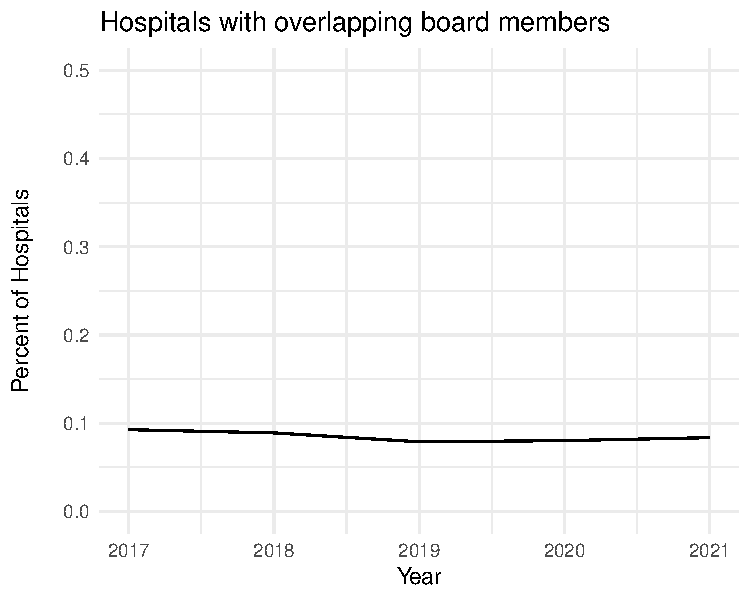
\includegraphics[width=.8\textwidth]{Objects/connected_percent.pdf}
        \label{fig:connected_percent}
    \end{figure}

    As mentioned previously, common board members should be more likely to affect hospital behavior within a hospital market, where hospitals compete for the same patient population. Of the 306 HRRs in the US, approximately 17\% have at least one pair of affiliated hospitals within the market. As shown in Figure \ref{fig:connected_HRR_percent}, this proportion decreases slightly over time, with 15\% of HRRs having connected hospitals in 2021, a nominal decrease of 8 markets losing hospitals with affiliation.  


    \begin{figure}[ht!]
        \centering
        \caption{Percent of HRRs containing board affiliated hospitals}
        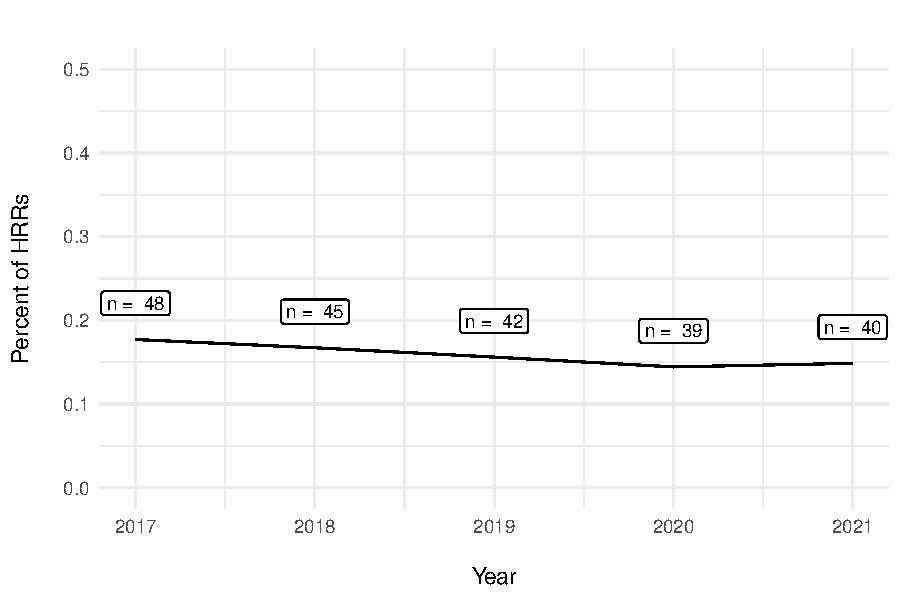
\includegraphics[width=.8\textwidth]{Objects/connected_HRR_percent.pdf}
        \label{fig:connected_HRR_percent}
    \end{figure}

    The geographic distribution of these pairs is shown in Figure \ref{fig:connected_maps}, where the blue dots represent hospitals that share a common board member. Connected hospitals are distributed fairly regularly across the US, apart from relatively few connections on the west coast relative to the population. Over time, the connections remain fairly consistent geographically.

    \begin{figure}[ht!]
        \centering
        \caption{Geographic distribution of board affiliated hospitals over time}
        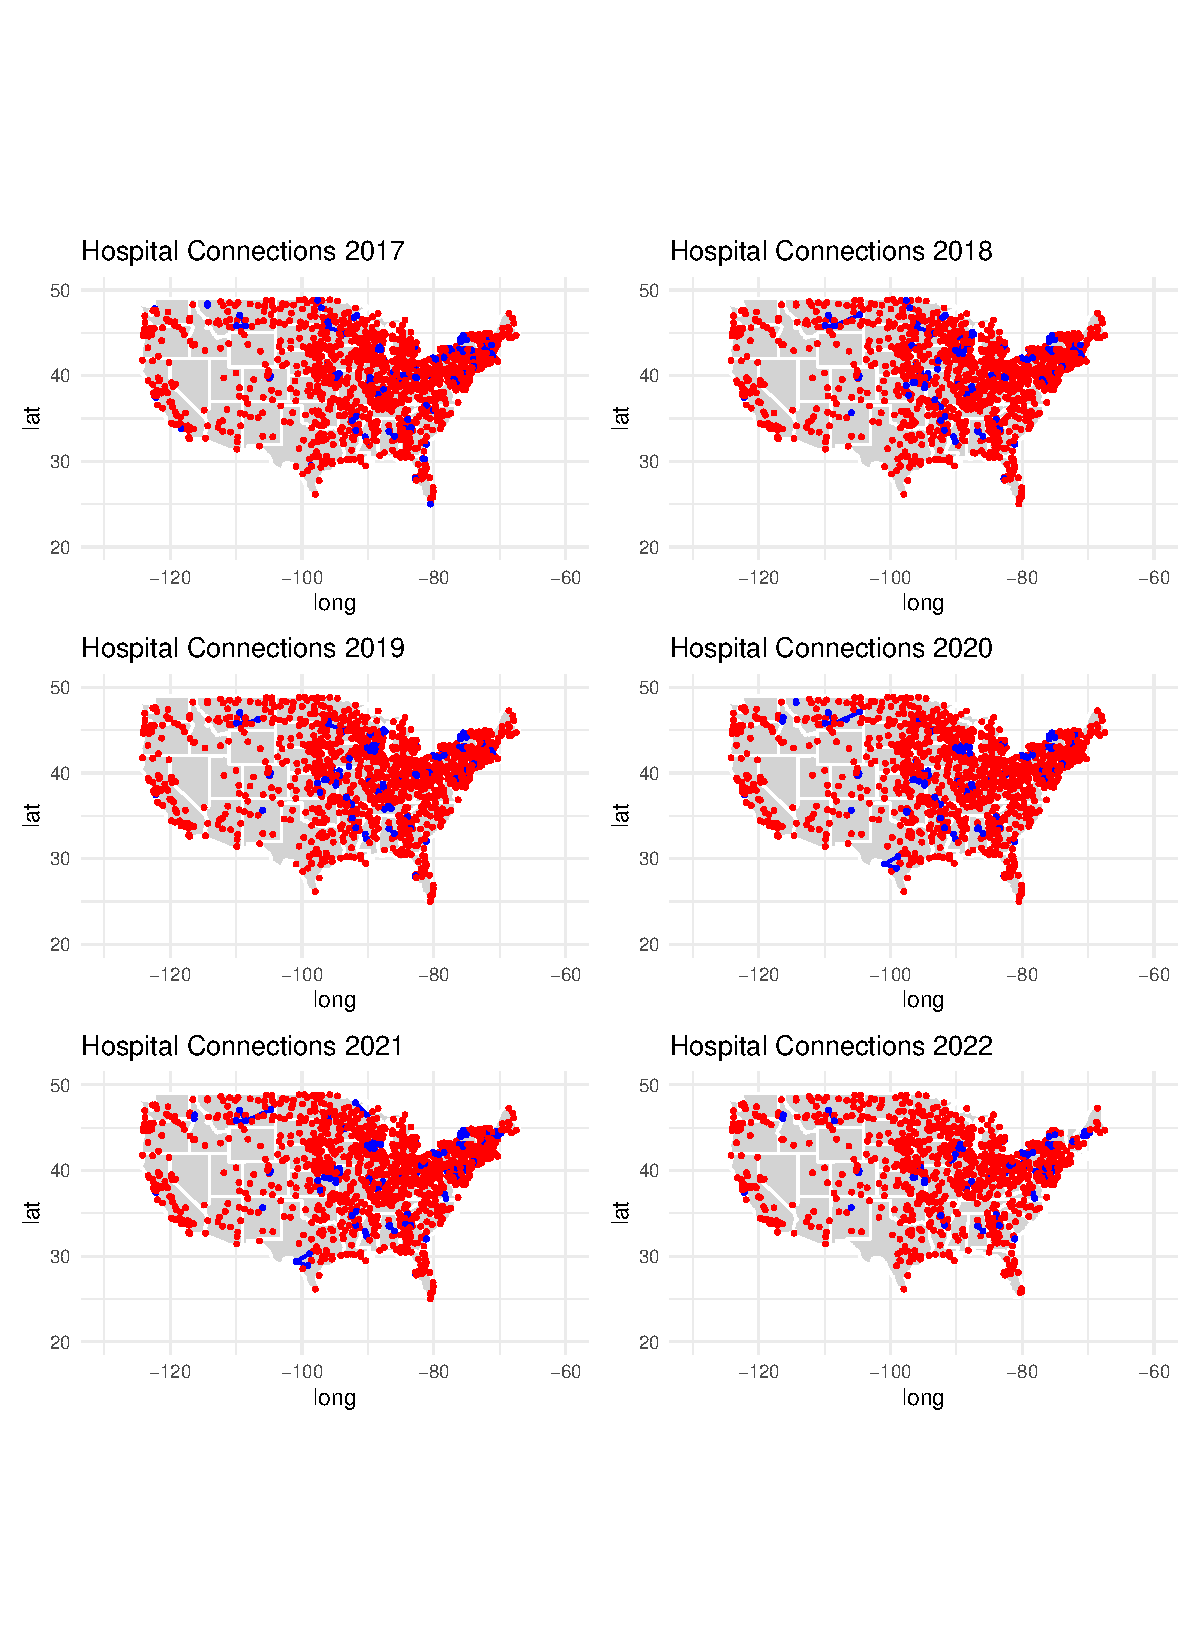
\includegraphics[width=.8\textwidth]{Objects/connected_maps.pdf}
        \label{fig:connected_maps}
    \end{figure}



    Next, I show the proportion of the type of hospital affiliations. Each hospital is general or specialty, children or adult, and independent or system, all characteristics found in the AHA data. In Table \ref{tab:hospital_pair_types}, I show that the majority of pairs are both general hospitals, and that there is significant variation in the ownership type of pairs. Forty-five percent of pairs are between two non-system affiliated hospitals, and 36\% of pairs are between an independent hospital affiliated with a hospital belonging to a system. 

    \import{Objects}{hospital_pair_types.tex}

    I now shift towards examining summary statistics of hospitals with different types of affiliation relationships. First, in Table \ref{tab:hospital_general_summarystats}, I focus on general hospitals in four categories: affiliated through shared board members with another general hospital, affiliated through shared board members with a specialty hospital, unaffiliated through board members but belonging to a system, and unaffiliated with other hospitals by board or system. I present means of hospitals in each of these categories for the number of beds, the number of patients seen, whether it is an academic medical center, and whether the hospital is located in a metropolitan area. On these dimension, the hospital affiliated with other general hospitals (1) are relatively similar to unaffiliated hospitals that are part of a system (3). Unaffiliated hospitals that are not part of a system are slightly smaller in terms of bed size and number of patients seen, and less likely to be in a metropolitan area. The hospitals in column (2) are outliers, with a large number of beds and patients seen, and mainly in metropolitan areas. There are only 12 hospitals in this sample that are likely very different from the average hospital. 

    \import{Objects}{hospital_general_summarystats.tex}

    I also present means of variables to capture aspects of the service offerings of the different types of hospitals. First, from the AHA survey, I include an indicator for whether the hospital offers services in a Neonatal Intensive Care Unit (NICU) or Cardiac catheterization lab, both specialized and profitable services. General hospitals that are affiliated with specialty hospitals are the most likely to offer these services. Hospitals without any board member affiliations but belonging to a system are more likely to offer these services than unaffiliated hospitals that do not belong to a system. Hospitals that are affiliated with another general hospitals fall somewhere in between these two, with slightly less likelihood than the unaffiliated hospitals belonging to a system. 

    I also include a measure of the concentration of services offered by the hospital using a Herfindahl-Hirschman Index calculation of the number of beds devoted to each service category in the AHA data. Specifically, for each hospital, I compute the proportion of total beds assigned to each service category and then square these proportions before summing them. A higher HHI value indicates that a hospital's bed capacity is concentrated in fewer service categories, whereas a lower HHI suggests a more diversified service offering, which provides insight into the degree of specialization or diversification in a hospital’s service provision. I also compute a similar concentration metric using the percent of patients in several service categories from the CMS Provider Utilization Files, including cancer, Chronic Obstructive Pulmonary Disease (COPD), kidney, and heart-related services. For both measures, the variation in service concentration is low across affiliation types, with the most concentrated hospitals being those unaffiliated through board members. 

    Next, I present the same summary statistics for specialty hospitals with different types of affiliations: affiliated with a general hospital, unaffiliated through board but belonging to a system, and unaffiliated through board or system, shown in Table \ref{tab:hospital_specialty_summarystats}. Overall, there are less specialty hospitals included in the sample, and very few of them are affiliated through board members. Specialty hospitals are more concentrated than general hospitals, as expected. In the AHA measure of concentration, all specialty hospitals are similarly concentrated. However, when using the services included in the CMS files, the concentration of unaffiliated system hospitals is much lower than that of any other specialty hospital. This could be due to the limited services included in the CMS data. 

    \import{Objects}{hospital_specialty_summarystats.tex}

    In Figure \ref{fig:concentration_services_time}, I show the AHA measure of service concentration based on the number of beds over time for general hospitals with different levels of affiliation. General hospitals that are unaffiliated through board members, whether they are affiliated with a system or not, remain relatively constant in their service offerings over time. However, general hospitals that are affiliated with another general hospital through a shared board member display increasing service concentration over time, suggesting that there may be some correlation between board affiliations and the services offered in hospitals.  

    \begin{figure}[ht!]
        \centering
        \caption{Concentration of services offered over time}
        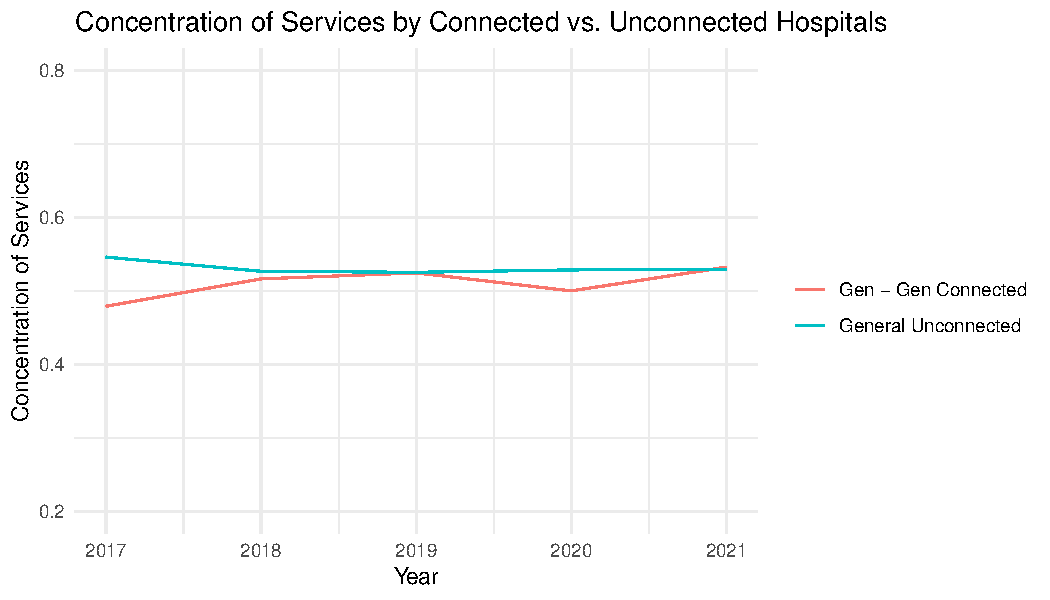
\includegraphics[width=0.8\textwidth]{Objects/concentration_services_time.pdf}
        \label{fig:concentration_services_time}
    \end{figure}

    \newpage


    \printbibliography


    

    

    

    

    

	
	
	


\end{document}

